\chapter{Distributed Safe Bayesian Optimization}
\label{ch:distbo}

\section{System Model and Problem Statement}
We will be given with an unknown function $f: \mathcal{X} \to \mathbb{R}$ over some domain $\mathcal{X} \subset \mathbb{R}^d$. But $f$ is expensive to compute and no access to gradients.
The objective of the safe optimization problem is to find the maximum of an unknown function $f(x)$ where $x \in \mathcal{X}$ subject to safety constraints. 
We assume that $f(x)$ is a Lipschitz continuous function of $x$ on a compact set $\mathcal{X}$. The Lipschitz constant is assumed to be $L$.
Furthermore, the seed set $S_0 \subset \mathcal{X}$ that contains atleast one safe point. 
We should ensure that, for all time steps $t$, it holds that $f(x_t) \geq h$, where $h$ is a problem-specific safety threshold.
We can divide each search space dimension into $n$ number of subspaces and take the all possible combinations to form $n^d$ hyperspaces. Thus we assume that there are $m \ge n^d$ computing nodes avialable. 
Additionally, we will be having time and communication constraint for a given network connection.

We note that since the function is unknown, we optimize the function by observing the value of the function at points $x_t \in \mathcal{X}$ which are chosen for every time $t$, meeting the safety constraint $f(x_t) \geq h$.
So our problem is to find safely reachable point $x^* \in \mathcal{X}$ which maximizes the value of our unknown function $f$, by distributing the computation possibly among $m$ nodes by deploying safely reachable hyperspace in each node.

\section{Distributed SafeOpt}
For a given search space $\mathcal{X}$ with $d$ search dimensions(parameters) and $n$ number of subspaces per parameter, we can take the all possible combination of subspaces to create hyperspaces. So $n^d$ hyperspaces are possible. 
We start the optimization process in a single node for a given objective function $f$, search space $\mathcal{X}$, and safe set $S_0$. 
We take the hyperspace to which initial safe points in set $S_0$ belong as the \textit{currently deployed hyperspace}. 
We check whether that point $x_{next}$ belongs to the new non-deployed hyperspace for the sampled new point. 
If so, we check the function value $f(x_{next}) \geq h$ for safety constraint violation. 
The points that do not meet the safety constraint are considered unsafe evaluations and are stored into the evaluated points array and will be used to define prior in the upcoming search space splitting procedure.
The point that meets safety constraints splits the present search space between \textit{current-hyperspace} and \textit{new-hyperspace}. 
The point $x_{next}$ will be the safe seed for new search space that contains \textit{new-hyperspace} and we start optimization for this in a new node. 
The $S_0 \cup \{ \text{any other safe point evaluated in }\textit{current-hyperspace } \}$ will be the safe seed for other search space that contains \textit{current-hyperspace} and the optimization process will be restarted in the same node with updated search space bounds. 
Repeat the same procedure to successively divide the search space into a single hyperspace (leaf node). Algorithm \ref{alg:dsbo} explains the initialization of optimization process, and algorithm \ref{alg:deployhs} recursively instiates the new optimization nodes, uses \texttt{SafeOpt} \ref{alg:safeopt} for safe optimization.

\begin{algorithm}[h!]
%	\SetAlgoVlined
	\caption{Distributed SafeOpt}
	\label{alg:dsbo}
	\KwIn{Objective function $f$, GP prior($\mu, k$), Parameter search-space $\mathcal{X}$, Number of parameters $d$, Number of subspaces per parameter $n$, Safe seed set $S_0$, Safety threshold $h$}
	\ForEach{$parameter$ in $\mathcal{X}$}
	{
		divide $parameter$ into $n$ subspaces.
	}
	Take all possible combination of subspaces to form $hyperspaces$.\\
	currentSafeHyperspace = $hyperspace : allHyperspaces | S_0 \in hyperspace$\\
	Deploy optimization process for whole search-space into a single node.\\		
\end{algorithm}

\begin{algorithm}[h!]
%	\SetAlgoVlined
	\caption{Deploy Hyperspace}
	\label{alg:deployhs}
	\KwIn{$f$, GP($\mu, k$), $\mathcal{X}$, $S_0$, $h$, $currentSafeHyperspace$, $allHyperspaces$}
	Initialize \texttt{SafeOpt} with safe seed points $S_0$.\\
	\If{currentSafeHyperspace $is$ leafHyperspace}
	{
		\For{$i=1:\dots$}
		{
			run \texttt{SafeOpt} algorithm
		}
		\KwRet{}
	}
	\For{$i=1:\dots$}
	{
		samplePoint=\texttt{SafeOpt}.optimize()\\
		funcValue=$f$(samplePoint)\\
		newSafeHyperspace = hyperspace : allHyperspaces | samplePoint $\in$ hyperspace\\
		\eIf{funcValue $\ge h$ AND newSafeHyperspace $\neq$ currentSafeHyperspace}
		{
			Split the search space between two hyperspaces.\\
			Deploy the newSafeHyperspace into new node with samplePoint as safe seed.\\
			Change the search space for currentSafeHyperspace accordingly and continue optimization process in same node.\\
		}
		{
			add samplePoint and funcValue to \texttt{SafeOpt} model.
		}
		
	}
\end{algorithm}

\subsection{Example Discussion}
Figure \ref{fig:dsbo-example} shows a 2-dimensional search space example for which \textit{Distributed SafeOpt} is applied for optimization. 
$H1$ nad $H2$ are two dimensions of search space with bounds $(-8, 8)$ and $(-8, 8)$ respectively. 
Here we are dividing each dimension into 4 subspaces, so total $2^4=16$ hyperspaces are possible i.e., combination of subspace-2 of $H1$ and subspace-3 of $H2$ is hyperspace-11. 
The point in the safe seed $S_0$ belongs to hyperspace-10. 
Used green and red color to represent safe and unsafe evaluations of the algorithm respectively. 
Figure \ref{fig:dsbo-example-a} shows initial state of the optimization, where safe seed in hyperspace-10, this is deployed into node-0. 
Figure \ref{fig:dsbo-example-b} shows a newly sampled safe point in hyperspace-15, so the search space is split between hyperspace-10 and hyperspace-15 as shown in figure \ref{fig:dsbo-example-c} with different colors.
So the first search space has bounds $[(-8,4), (-8,8)]$ with safe seed in hyperspace-10. Similarly, the second search space hs bounds $[(4,8),(-8,8)]$ with safe seed in hyperspace-15.
This second search space is deployed into a new node node-1, whereas the first search space is redeployed in the same node node-0.

Now, we have two optimization processes at two different nodes, which independently samples next points of interest and follow the algorithm to split the search space as required.
One thing to notice in node-1, (see figure \ref{fig:dsbo-example-d} right side search space) the next point sampled is unsafe, so the search space splitting will not happen until a safe point in some other hyperspace is found.
Once the search space bounds reduce to a single hyperspace bounds like hyperspace-15 in figure \ref{fig:dsbo-example-f}, we consider it as a leaf node and no further splitting of search space will happen.\\


\begin{figure}
	\centering
	\begin{subfigure}{0.45\textwidth}
		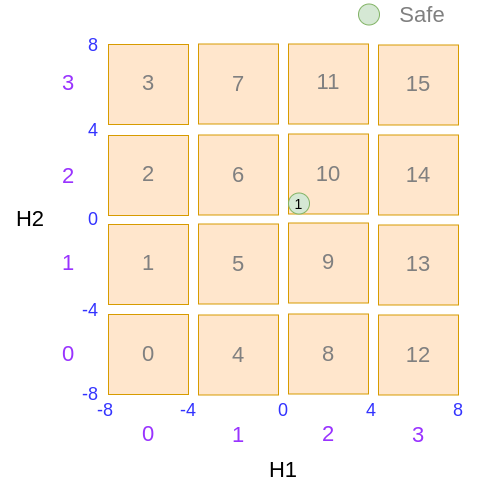
\includegraphics[width=0.8\textwidth]{figures/draw/a.png}
		\caption{}
		\label{fig:dsbo-example-a}
	\end{subfigure}
%	\hfill
	\begin{subfigure}{0.45\textwidth}
		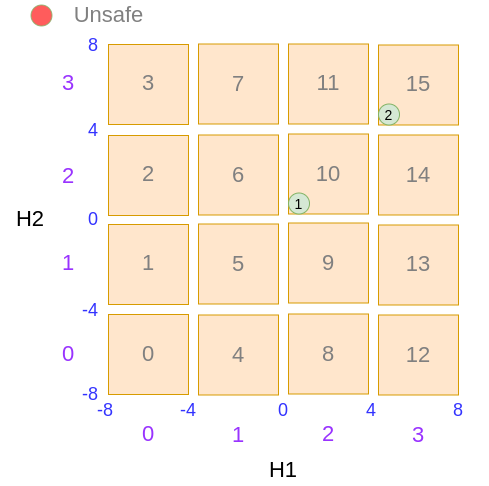
\includegraphics[width=0.8\textwidth]{figures/draw/b.png}
		\caption{}
		\label{fig:dsbo-example-b}
	\end{subfigure}
	\begin{subfigure}{0.45\textwidth}
		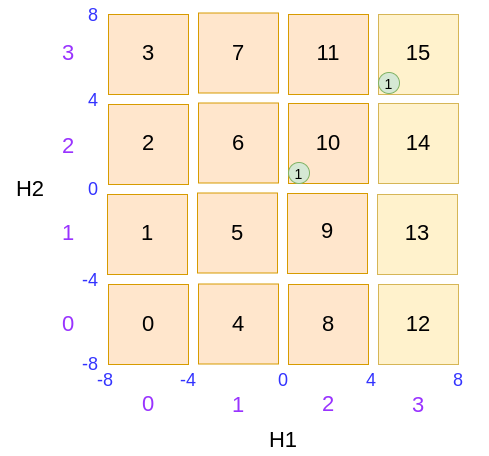
\includegraphics[width=0.8\textwidth]{figures/draw/c.png}
		\caption{}
		\label{fig:dsbo-example-c}
	\end{subfigure}
	\begin{subfigure}{0.45\textwidth}
		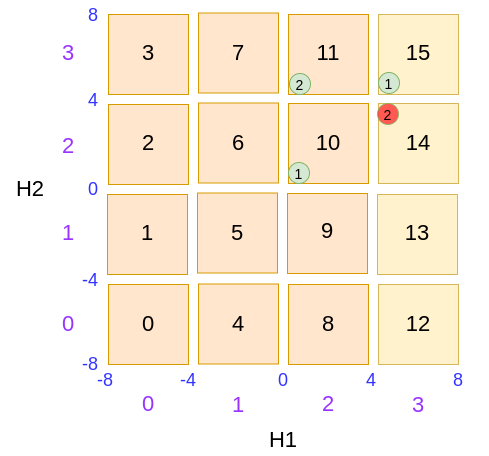
\includegraphics[width=0.8\textwidth]{figures/draw/d.png}
		\caption{}
		\label{fig:dsbo-example-d}
	\end{subfigure}
	\begin{subfigure}{0.45\textwidth}
		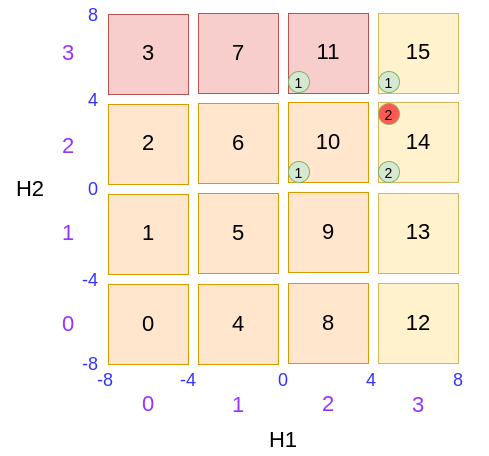
\includegraphics[width=0.8\textwidth]{figures/draw/e.png}
		\caption{}
		\label{fig:dsbo-example-e}
	\end{subfigure}
	%	\hfill
	\begin{subfigure}{0.45\textwidth}
		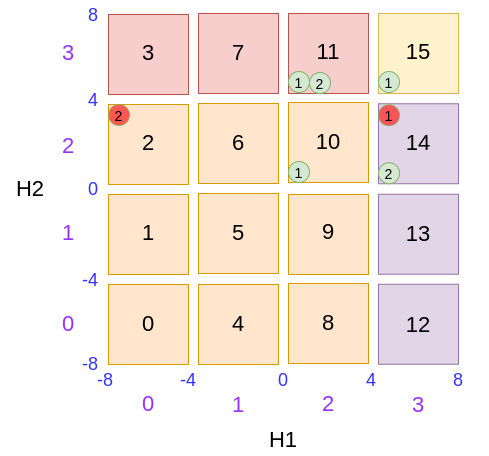
\includegraphics[width=0.8\textwidth]{figures/draw/f.png}
		\caption{}
		\label{fig:dsbo-example-f}
	\end{subfigure}
	\begin{subfigure}{0.45\textwidth}
		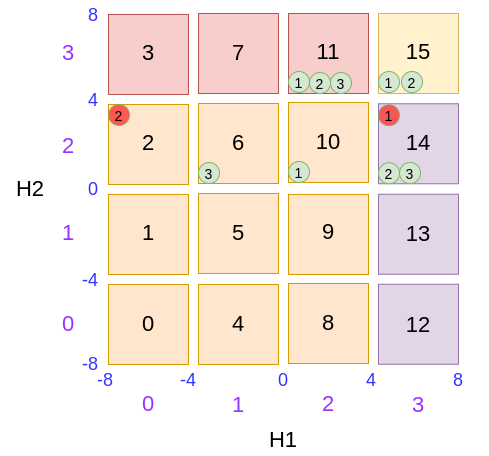
\includegraphics[width=0.8\textwidth]{figures/draw/g.png}
		\caption{}
		\label{fig:dsbo-example-g}
	\end{subfigure}
	\begin{subfigure}{0.45\textwidth}
		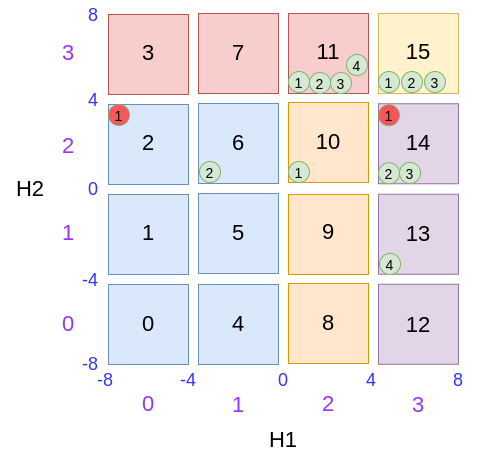
\includegraphics[width=0.8\textwidth]{figures/draw/h.png}
		\caption{}
		\label{fig:dsbo-example-h}
	\end{subfigure}
	\caption{Illustration of algorithm for a 2-dimensional search space example}
	\label{fig:dsbo-example}
\end{figure}

\section{Test Setup}
We are running our algorithm on standard optimization functions (Bird function, Langermanns' function, Lavy05 function, and Michalewicz's function) to test the performance in terms of achievable maximum and cumulative unsafe evaluations. 
The performance is compared with \texttt{SafeOpt} algorithm as baseline. Details are discussed in following subsections.
\subsection{Bird Function}
Bird function is a 2-dimensional unimodal function, defined as
$$ f(x, y) = \sin(y) \exp (1-\cos(x))^2 + \cos(x)\exp(1-\sin(y))^2 + (x - y)^2. $$
Search space is $ [ (-2\pi, 2\pi), (-2\pi, 2\pi) ] $. And global minima is $f^*=-106.764537$ found at $(x_1, y_1)=(4.70104, 3.15294)$ and $(x_2, y_2)=(-1.58214, -3.13024)$.
\begin{figure}
	\centering
	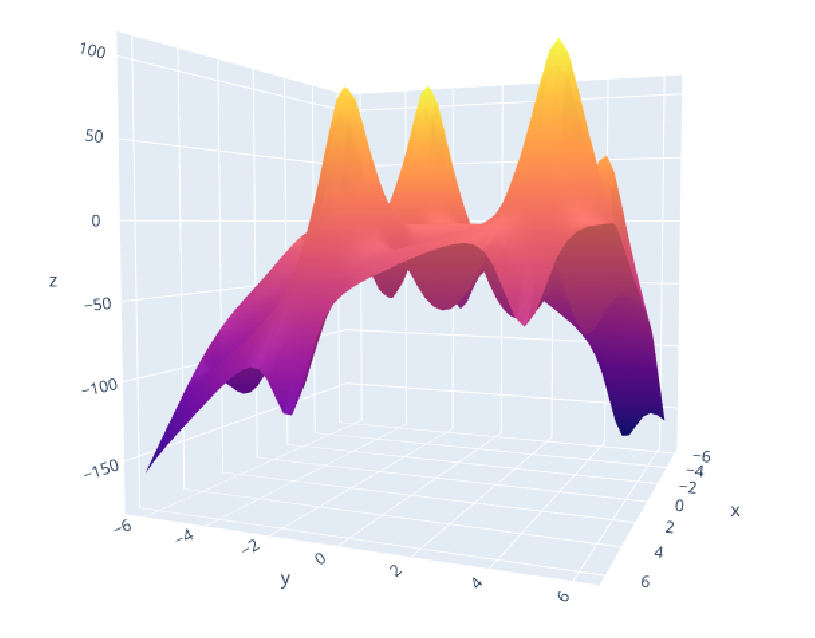
\includegraphics[scale=0.4]{figures/bird-function-plot.png}
	\caption{Bird function plot.}
	\label{fig:bird-function-plot}
\end{figure}
Figure \ref{fig:bird-function-plot} shows the view of the function.

\subsection{Langermanns' Function}
The Langermann function is a multimodal test function. The local minima are unevenly distributed.
And is defined as $$ f(x,y) = \sum_{i=1}^{m}c_i \exp(-(x-a_i)^2 / \pi - (y - b_i)^2 / \pi) \cos(\pi (x-a_i)^2 + \pi (y - b_i)^2) $$
We are considering the case where $m=5$ and $a=[3, 5, 2, 1, 7],$ $b = [5, 2, 1, 4, 9],$ and $c = [1, 2, 5, 2, 3]$. Search space is $[(3, 5), (3, 5)]$.
\begin{figure}
	\centering
	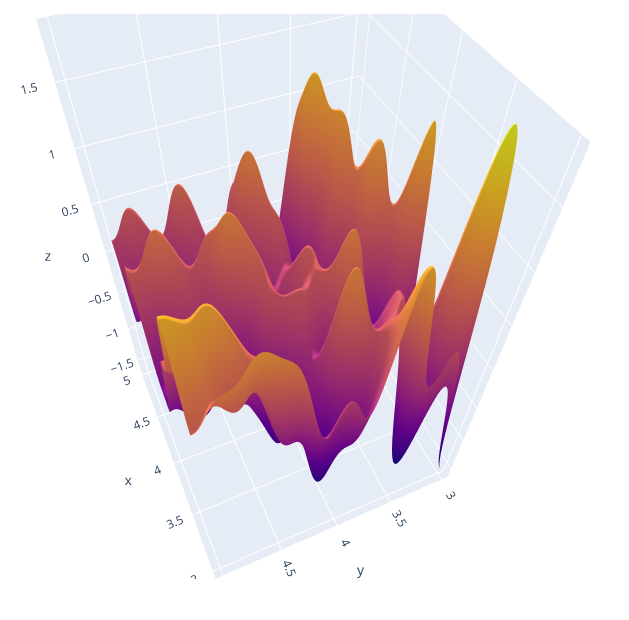
\includegraphics[scale=0.4]{figures/langermann-function-plot.png}
	\caption{Langermann function plot.}
	\label{fig:langermann-function-plot}
\end{figure}
Figure \ref{fig:langermann-function-plot} shows the view of the function.

\subsection{Levy05 Function}
This is a multimodal optimization problem. Defined as
$$ f(x,y) = \sum_{i=1}^{5} i \cos[(i-1)x + i] \times \sum_{j=1}^{5} j \cos[(j+1)y+j] + (x+1.42513)^2 + (y+0.80032)^2 $$
Search space is $[(-2, 2), (-2, 2)]$. And global minima is $f^*=176.1375$ at $(x, y)=(-1.3068, -1.4248)$. 
\begin{figure}
	\centering
	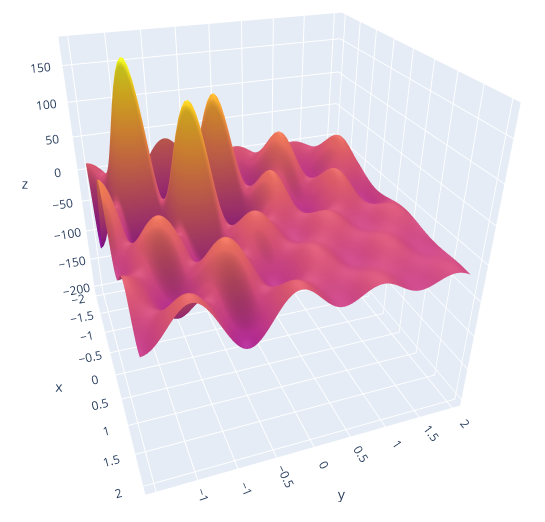
\includegraphics[scale=0.5]{figures/levy05-function-plot.png}
	\caption{Levy05 function plot.}
	\label{fig:levy05-function-plot}
\end{figure}
Figure \ref{fig:levy05-function-plot} shows the view of the function.

\subsection{Michalewicz's function}
The Michalewicz function is a multimodal test function (owns $n!$ local optima).
The parameter $m$ defines the steepness of the valleys or edges. 
Larger $m$ leads to more difficult search. 
For very large $m$ the function behaves like a needle in the haystack (the function values for points in the space outside the narrow peaks give very little information on the location of the global optimum). 
Function has the following definition
$$ f(x) = -\sum_{i=1}^{n}\sin(x_i) \left[ \sin(\frac{ix_i^2}{\pi}) \right]^{2m}  $$
It is usually set $m=10$. Test area is usually restricted to hyphercube $0 \leq x_i \leq \pi,\ i = 1, \dots, n$. The global minimum value has been approximated by $f(x)=-4.687$ for $n=5$ and by $f(x)=-9.66$ for $n=10$.
Respective optimal solutions are not given.

\newpage
\section{Results}
\subsection{Bird Fuction}
Figure \ref{fig:bird-result} shows a sample run on Bird function. Noise variance is $0.05^2$, RBF kernel (var=2, lengthscale=1) as prior and $S_0=\{ (0,0) \}$.
\begin{figure}[h!]
	\centering
	\begin{subfigure}{0.99\textwidth}
		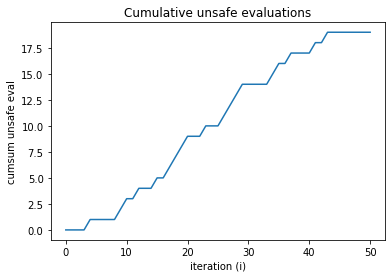
\includegraphics[width=0.48\textwidth]{figures/results/bird-sbo-cum-unsafe.png}
		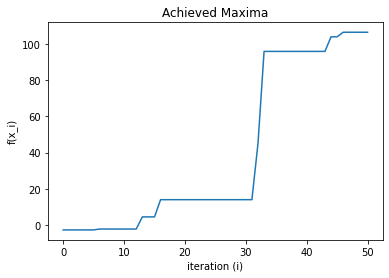
\includegraphics[width=0.48\textwidth]{figures/results/bird-sbo-maxima.png}
		\caption{SafeOpt run}
		\label{fig:bird-result-sbo}
	\end{subfigure}
	\vfill
	\begin{subfigure}{0.98\textwidth}
		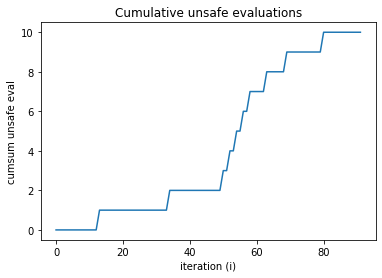
\includegraphics[width=0.48\textwidth]{figures/results/bird-dbo-cum-unsafe.png}
		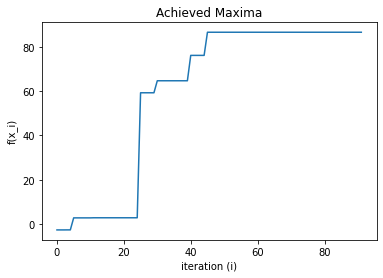
\includegraphics[width=0.48\textwidth]{figures/results/bird-dbo-maxima.png}
		\caption{Distributed SafeOpt run}
		\label{fig:bird-result-dbo}
	\end{subfigure}
	\caption{Bird function results}
	\label{fig:bird-result}
\end{figure}

\newpage
\subsection{Langermann's Fuction}
Figure \ref{fig:langermann-result} shows a sample run on Langermann's function. Noise variance is $0.25^2$, RBF kernel (var=2, lengthscale=1) as prior and $S_0=\{ (4.3,4.3) \}$.
\begin{figure}[h!]
	\centering
	\begin{subfigure}{0.99\textwidth}
		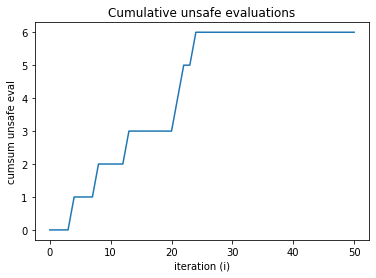
\includegraphics[width=0.48\textwidth]{figures/results/langermann-sbo-cum-unsafe.png}
		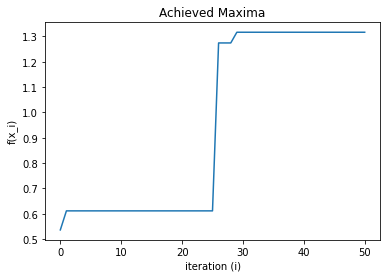
\includegraphics[width=0.48\textwidth]{figures/results/langermann-sbo-maxima.png}
		\caption{SafeOpt run}
		\label{fig:langermann-result-sbo}
	\end{subfigure}
	\vfill
	\begin{subfigure}{0.98\textwidth}
		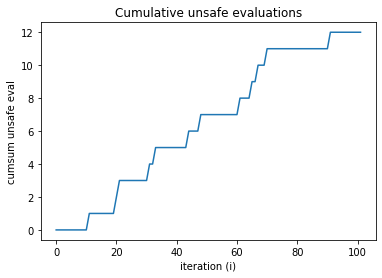
\includegraphics[width=0.48\textwidth]{figures/results/langermann-dbo-cum-unsafe.png}
		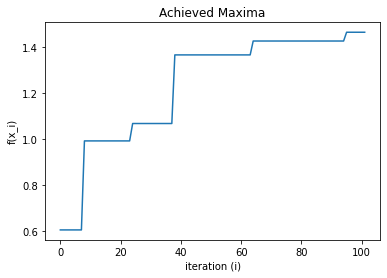
\includegraphics[width=0.48\textwidth]{figures/results/langermann-dbo-maxima.png}
		\caption{Distributed SafeOpt run}
		\label{fig:langermann-result-dbo}
	\end{subfigure}
	\caption{Langermann's function results}
	\label{fig:langermann-result}
\end{figure}

\newpage
\subsection{Levy05 Fuction}
Figure \ref{fig:langermann-result} shows a sample run on Levy05 function. Noise variance is $0.05^2$, RBF kernel (var=5, lengthscale=1) as prior and $S_0=\{ (0.5, 0.2) \}$.
\begin{figure}[h!]
	\centering
	\begin{subfigure}{0.99\textwidth}
		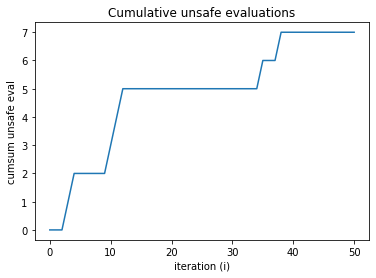
\includegraphics[width=0.48\textwidth]{figures/results/levy05-sbo-cum-unsafe.png}
		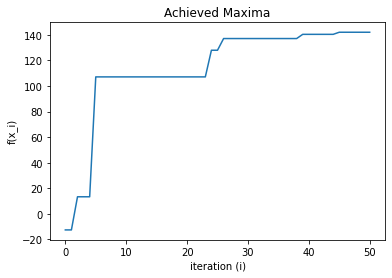
\includegraphics[width=0.48\textwidth]{figures/results/levy05-sbo-maxima.png}
		\caption{SafeOpt run}
		\label{fig:levy05-result-sbo}
	\end{subfigure}
	\vfill
	\begin{subfigure}{0.98\textwidth}
		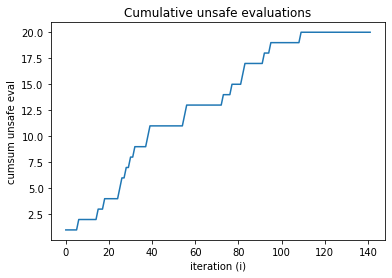
\includegraphics[width=0.48\textwidth]{figures/results/levy05-dbo-cum-unsafe.png}
		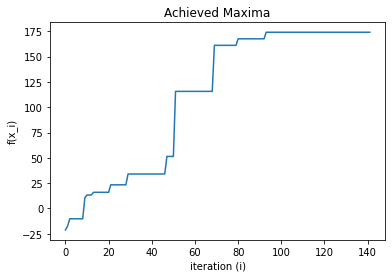
\includegraphics[width=0.48\textwidth]{figures/results/levy05-dbo-maxima.png}
		\caption{Distributed SafeOpt run}
		\label{fig:levy05-result-dbo}
	\end{subfigure}
	\caption{Levy05 function results}
	\label{fig:levy05-result}
\end{figure}

\newpage
\subsection{Michalewicz Fuction}
Figure \ref{fig:langermann-result} shows a sample run on Michalewicz function. Noise variance is $0.05^2$, RBF kernel (var=2, lengthscale=1) as prior and $S_0=\{ (2, 3, 1, 2, 3) \}$.
\begin{figure}[h!]
	\centering
	\begin{subfigure}{0.99\textwidth}
		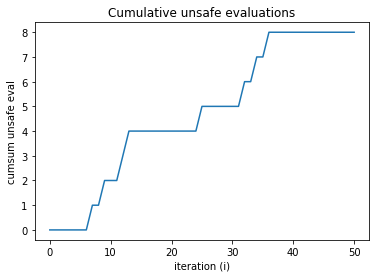
\includegraphics[width=0.48\textwidth]{figures/results/michalewicz-sbo-cum-unsafe.png}
		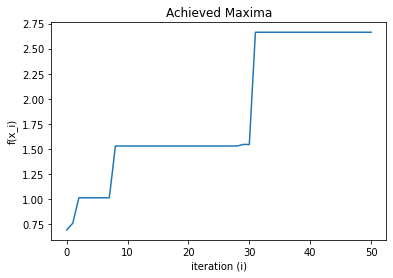
\includegraphics[width=0.48\textwidth]{figures/results/michalewicz-sbo-maxima.png}
		\caption{SafeOpt run}
		\label{fig:michalewicz-result-sbo}
	\end{subfigure}
	\vfill
	\begin{subfigure}{0.98\textwidth}
		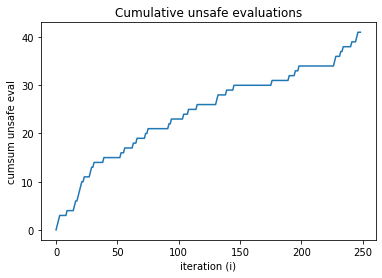
\includegraphics[width=0.48\textwidth]{figures/results/michalewicz-dbo-cum-unsafe.png}
		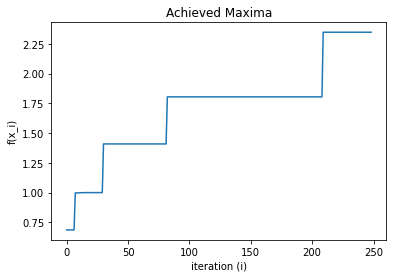
\includegraphics[width=0.48\textwidth]{figures/results/michalewicz-dbo-maxima.png}
		\caption{Distributed SafeOpt run}
		\label{fig:michalewicz-result-dbo}
	\end{subfigure}
	\caption{Michalewicz function results}
	\label{fig:michalewicz-result}
\end{figure}